\chapter{Does life history mediate changing disease risk when communities disassemble?}
\chapterauthor{Maxwell B. Joseph, Joseph R. Mihaljevic, Sarah A. Orlofske, and Sara H. Paull}
\label{ch2}

Biodiversity loss sometimes increases disease risk or parasite transmission in humans, wildlife and plants. Some have suggested that this pattern can emerge when host species that persist throughout community disassembly show high host competence – the ability to acquire and transmit infections.
Here, we briefly assess the current empirical evidence for covariance between host competence and extirpation risk, and evaluate the consequences for disease dynamics in host communities undergoing disassembly. We find evidence for such covariance, but the mechanisms for and variability around this relationship have received limited consideration.
This deficit could lead to spurious assumptions about how and why disease dynamics respond to community disassembly.
Using a stochastic simulation model, we demonstrate that weak covariance between competence and extirpation risk may account for inconsistent effects of host diversity on disease risk that have been observed empirically.
This model highlights the predictive utility of understanding the degree to which host competence relates to extirpation risk, and the need for a better understanding of the mechanisms underlying such relationships.

\section{Introduction}

Biodiversity loss alters ecosystem functioning and services \citep{Cardinale2012}.
When local extinctions (extirpations) cause predictable losses of diversity, the consequences of local biodiversity loss are often non-random \citep{Henle2004, Cadotte2011}.
In disease ecology, there is an emerging idea that host diversity can reduce or ‘dilute’ disease risk, especially when diverse communities include species that reduce transmission due to low host competence – the ability to acquire and transmit infections \citep{Keesing2010}.
Whether diversity generally decreases disease risk due to a ‘dilution effect’ remains contentious partly due to uncertainty in whether host extirpation risk relates to host competence \citep{Randolph2012}.

Covariance between host competence and extirpation risk could arise due to host life-history trade-offs, parasite adaptation to locally common hosts, or both.
Host life-history trade-offs could operate if slow-lived species (e.g. those that are long-lived, large-bodied, and slowly reproducing) invest more heavily in parasite defence and experience higher extirpation risk, whereas fast-lived species invest little in parasite defence but are more ubiquitous in disassembled (or generally depauperate) communities \citep{Huang2013a}.
Alternatively, parasites could adapt to locally common hosts, which likely experience lower extirpation risk due to higher population densities \citep{Lively2000}.
These mechanisms are not mutually exclusive, and both have received empirical support.
However, the generality of these mechanisms remains uncertain, and the general consequences of resulting covariance between competence and extirpation risk have not been rigorously evaluated (but see \citet{Ostfeld2003} for a detailed system-specific evaluation).

To better understand how and why host diversity loss influences disease risk, we address three objectives: (1) clarify the rationale underlying extirpation risk-host competence relationships, (2) review the empirical evidence for these relationships and (3) evaluate the theoretical consequences for disease across a range of extirpation risk-host competence scenarios.
Finally, we present empirical methods for disentangling the mechanisms underlying covariance between host competence and extirpation risk, with the goal of more accurately predicting the effects of biodiversity loss on disease dynamics in natural systems.

\section{Determinants of Extirpation Risk}

A variety of species traits such as reproductive pace, body size and home range size have been linked to global extinction risk, and are likely also important for local extirpation risk.
Generally, large-bodied, slow-reproducing species recover more slowly from disturbances, and have low regional abundances which increases extirpation risk \citep{Damuth1981, Hanski1991, Nee1991, Cardillo2001, Meehan2004, Buckley2007, Davidson2009}.
Furthermore, average home range size is negatively correlated with density in many mammals, and positively correlated to body size in birds \citep{Bordes2009a, lee2011}, and as such, species with large home ranges and low population densities can experience higher extirpation risk \citep{Boyle2010}.
However, among species with small populations, long-lived species appear to experience lower extirpation risk than those that are fast lived \citep{Saether2011}.
Large body size, long lifespan, delayed maturity and specialised feeding behaviours can contribute to a higher frequency of local extirpation risk in fishes \citep{Olden2007}.
Finally, species at the highest trophic levels are often more prone to local extirpations due to demography and direct human impacts such as hunting \citep{Duffy2003}.
Such effects could lead to trophic cascades that influence not only species composition but also abundance in low diversity areas \citep{Hebblewhite2005}.

Ecological communities are often nested such that local species composition tends to be a nested-subset of the most species communities in a region \citep{Wright1998}.
Variation in habitat characteristics (i.e. extrinsic factors) as well as species traits (i.e. intrinsic factors) has been implicated in the emergence of nested patterns \citep{Almeida2007}.
The nested nature of many communities can also arise due to community disassembly at varying stages.
For example, in Amazonian primate and carnivore communities, forest fragmentation leads to nested communities due to species-specific effects of patch size on extirpation risk \citep{Michalski2005}.
To anticipate changes in host community competence as species are driven to local extinction, one could ask whether traits that mediate extirpation risk also mediate host competence.

\section{Determinants of Host Competence}

Host competence can be influenced by life-history trade-offs and parasite adaptation.
Work within the field of ecoimmunology has suggested that relationships between host competence and life history traits could arise because defence against infection leads to an increase in the host's future reproduction (via enhanced survival) at the expense of current reproduction \citep{Hawley2010}.
In other words, investment in current and future reproduction trade-off due to limited resource allocation to growth, maintenance and reproduction \citep{Stearns1992, Roff2001, Ricklefs2002}.
Therefore, individual investment in parasite defence is expected to co-vary with traits associated with survival and reproduction, such as body size, longevity and reproductive output \citep{Lee2006a, Cronin2010}.
This leads to the generalised prediction that fast-lived species invest less in immunological defences compared to slow-lived species (Figure \ref{2-1}; \cite{Cronin2010, Johnson2012}).
Such relationships between host competence and life history have been documented in the hosts of \textit{Borrelia burgdorferi} (the causative agent of Lyme disease), West Nile Virus (Huang et al. 2013), trematode parasites (Johnson et al. 2012, 2013) and Kissing bugs (\textit{Rhodnius pallescens}) that transmit \textit{Trypanosoma cruzi} infections \citep{Gottdenker2012}.
Host–parasite interactions (e.g. differential evasion of host immunity by parasites in a host community) could add variance to the relationship between investment in defence and realised host competence (Figure \ref{2-1}; \cite{Grenfell2004}).
Nonetheless, it is reasonable to assume that increased investment in defence reduces host competence on average.

Parasite evolution provides another mechanism for the relationship between host traits and infection.
Across host–pathogen systems, parasites exhibit local adaption to common host species and genotypes \citep{Kaltz1998, Lively2000, Lajeunesse2002, Montarry2008}.
Likewise, due to the selective pressure of losing hosts during community disassembly, parasites that exploit multiple hosts may evolve to infect the most abundant or widespread hosts leading to the negative relationship between extirpation risk and host competence.
Local adaptation of pathogens has received relatively limited attention in discussions of diversity-disease relationships to date despite being suggested as a possible mechanism for disease dilution over a decade ago \citep{ostfeld2000biodiversity}.

\section{Covariance Between Extirpation Risk and Host Competence}

Empirical evidence for competence-extirpation risk covariance is building.
For three vector-borne disease systems, host species with fast life histories (e.g. small body size) that tend to experience lower extirpation risk are better able to acquire and transmit infections than slow-lived host species \citep{Huang2013a}.
Similarly, fast-lived amphibians and those that are more abundant in species poor communities experience higher infection risk and more severe pathology from trematode parasites \citep{Johnson2012, Johnson2013}.
This pattern appears relevant to zoonotic diseases as well: widely distributed primates with dense populations are more likely to transmit parasites to other species, including humans \citep{Gomez2013}.
Still, departures from strict scaling between extirpation risk and host competence have been reported.
A recent empirical study of primates did not detect statistically significant covariance between susceptibility to habitat disturbance and parasite prevalence – a candidate proxy for host competence assuming constant parasite exposure \citep{Young2013}.
Even when statistically significant relationships are detected, many papers report substantial variance in competence not explained by life history, which is to be expected due to imperfect covariance between investment in immunity and realised competence (Figure \ref{2-1}; \cite{Johnson2012, Huang2013}).

The general consequences of competence-extinction risk relationships have not been rigorously explored, despite being framed as an assumption and possible mechanism of the dilution effect \citep{Randolph2012, Huang2013, Young2013}.
Beginning with an understanding from limited existing empirical data that there may be strong, weak or no correspondence between competence and extirpation risk, we built a model to explore how disease dynamics change as communities are disassembled under these possible scenarios.
We predicted that strong negative covariance between extirpation risk and host competence would lead in most cases to dilution effects, because poor hosts are extirpated early in community disassembly, consistent with previous studies that have made this assumption \citep{Roche2012}.
As this covariance became weaker, we expected that the effects of species extirpations on disease risk would become more variable.
Finally, we predicted that strong positive covariance (competent species experience higher extirpation risk) would tend to cause increased disease risk following extirpations (amplification effects) as community disassembly favors less-competent hosts.

\section{Exploring the Consequences of Host Competence-Extirpation Risk Relationships}

\subsection{Model structure}

We represent transitions from susceptible, infectious and recovered individuals in a multi-host community with a generalised directly transmitted microparasite using a system of differential equations \citep{Dobson2004}:

\begin{eqnarray}
  \dfrac{S_i}{dt} = (b_i - \delta N_i)N_i - d_i S_i - S_i \sum_{j=1}^{N} \beta_{ij} I_j \\
  \dfrac{I_i}{dt} = S_i \sum_{j=1}^{N} \beta_{ij} I_j - I_i (d_i + v_i + \sigma_i) \\
  \dfrac{R_i}{dt} = \sigma_i I_i - d_i R_i \label{eq:sir}
\end{eqnarray}

where $S_i$, $I_i$ and $R_i$ represent the densities of susceptible, infectious and recovered individuals of species $i$.
Recovered individuals are assumed to have life-long protective immunity.
We assumed allometric scaling of host vital rates, disease-free equilibrium densities and infection induced death rates following established methods \citep{Leo1996, Dobson2004, Bolzoni2008a}.
Details for each parameter are provided in Table \ref{tab2}.

Host competence was represented by the probability of transmission given a contact between a susceptible and infectious individual, which is proportional to the intraspecific transmission rate $\beta_{ii}$ \citep{Keesing2006}.
Intraspecific transmission rates were calculated based on the potential for an epidemic in a naïve and isolated population (intraspecific $R_0$), recovery rates $\sigma_i$, pathogen-induced death rates $v_i$, background mortality rates $d_i$ and host densities at carrying capacity $K_i$ (Table \ref{tab2}).
Interspecific $R_0$ values were drawn from a right-skewed truncated gamma distribution so that populations of most species would not be readily invaded by the pathogen on their own, but some species would experience severe epidemics in the absence of other species, consistent with empirical evidence for multi-host pathogens \citep{Komar2003, Ostfeld2003, Huang2013, Johnson2013}.
With strict allometric scaling, intraspecific transmission rates ($\beta_{ii}$) were linearly and positively correlated with intraspecific $R_0$, and negatively related to body mass, so that small-bodied species were more competent than large-bodied species (Figure \ref{2-s1}).
Interspecific transmission between species $j$ and species $i$ ($\beta_{ij}$) was assumed to be symmetrical so that $\beta_{ij} = \beta_{ji}$, and was calculated as a scaled average of intraspecific transmission rates (Table \ref{tab2}; \cite{Dobson2004}).

We used a two-step approach to explore the degree to which host competence-extirpation risk relationships affect changes in disease risk during community disassembly.
First, we produced a gradient of communities spanning from the strict assumption of small-bodied species being most competent to the reverse assumption of small species being least competent. To achieve this, we first assumed reverse rank-ordering between body size and intraspecific $R_0$, so that smaller bodied species received the highest values of $R_0$ \citep{Roche2012, Roche2013}.
We then permuted the values of $R_0$ to produce all possible species-$R_0$ pairings, producing $N!$ unique communities all consisting of the same $N$ species, but with different species-$R_0$ pairings.
This created a gradient in the relationship between host competence and extirpation risk.
On one extreme, smaller species always have the highest generated values of $R_0$ (i.e. a strong, negative correlation between host competence and body size).
On the other extreme, smaller species always have lowest values of $R_0$.
Intermediate permutations represent a range of randomness (i.e. strength of covariance) from one extreme to the other, with maximum randomness occurring at the median number of inversions (Figure \ref{2-s2}).

Second, we explored the consequences of competence-extirpation risk relationships in the context of community disassembly by sequentially removing individual host species from each of the $N!$ communities generated in the previous step.
We varied the extirpation ‘rules’ to always, often or only rarely extirpate larger bodied species, gradually relaxing the empirically supported assumption that large-bodied (i.e. slow-paced) species have high extirpation risk.
Specifically, we assumed (1) deterministic extirpations of largest-bodied hosts, (2) semi-random extirpations with extirpation risk proportional to $1 − w_i^{-1}$ and (3) completely random extirpations, irrespective of body size.
The latter two methods represent partial and complete decoupling of extirpation risk and host competence.
A range of initial host community richness values were explored, but our results were not sensitive to initial richness, and computational cost increased rapidly as host species were added.
Thus, we present all model results with initial communities consisting of five species ($N = 5$).

We considered both compensatory and subtractive extirpations, corresponding to cases where persisting species do or do not increase in abundance following the extirpation of co-occurring species, respectively.
With density compensation, following an extirpation, remaining species increased in density in proportion to their original relative abundances so that community density remained fixed and independent of species richness \citep{MacArthur1972}.
Compensatory extirpations imply strong species interactions that result in host density regulation – one mechanism for dilution \citep{Keesing2006}.
Finally, in the interest of generality we considered both density-dependent transmission and frequency-dependent transmission, where host contact rates increase with or are independent of host densities, respectively.
Density-dependent transmission is often seen with directly transmitted diseases, and frequency-dependent transmission is common with vector-transmitted diseases \citep{McCallum2001}.
To capture general patterns emerging from the processes of randomly drawing intraspecific R0 values from a distribution, and when applicable extirpation stochasticity, we iteratively produced and disassembled N! communities 1000 times for each extirpation scenario, assuming either density-dependent transmission or frequency-dependent transmission.

For each community, we estimated disease risk as community-level R0, which is calculated as the dominant eigenvalue of the next-generation matrix \citep{Dobson2004}.
This matrix incorporates within-species and between-species transmission, as well as host species traits related to survival and reproduction.
Community $R_0$ is positively related to the maximum prevalence of infection in the host community.
Thus, using community $R_0$ as a measure of disease risk, we are able to incorporate both the ability of the pathogen to invade the host community, and the intensity of the resulting epidemic if invasion is possible.
We evaluate the effect of community disassembly by quantifying changes in disease risk resulting from species extirpations: the difference in community R0 before and after a species has been extirpated ($\Delta R_0$).
When a species is removed and $\Delta R_0$ is positive, removing that particular species increases community-level disease risk; the opposite would be true if $\Delta R_0$ is negative.
Simulations were conducted with R version 3.0.1 (R Core Team 2013).

\section{Results}

As the assumption of perfect covariation between competence and extirpation risk was relaxed by permutation and/or stochastic extirpations, the effect of species extirpations on disease risk quickly became more variable, exhibiting both dilution- and amplification-effect behaviour in most cases.
When large species were less competent and deterministically lost early in disassembly, dilution effects were observed in all cases except density-dependent transmission with subtractive extirpations (for which dilution effects are impossible).
Even with deterministic extirpations, when the relationship between competence and life history was relaxed by permutation, both dilution and amplification effects could be observed for most cases as the variance in $\Delta R_0$ increased rapidly (Figure \ref{2-2}).
In general, large changes in disease risk following extirpations became more common across all cases when there was imperfect correspondence between life history and host competence (Figure \ref{2-2}).

With semi-random extirpations of large-bodied hosts, slight relaxation of the relationship between competence and life-history caused large increases in the overall variance in $\Delta R_0$ so that both dilution and amplification effects were seen under most cases (Figure \ref{2-2}).
However, as the relationship between competence and life history became more random, the increase in variance in $\Delta R_0$ was less pronounced for these semi-random extirpations than in the case of deterministic extirpations.
With completely random extirpations, the overall variance in $\Delta R_0$ was maximised, with a slight bias towards dilution, but with dilution and amplification nearly equiprobable regardless of the relationship between host competence and life history (Figure \ref{2-s3}).
When large-bodied species were more competent than small-bodied species and lost early in community disassembly, mixed amplification and dilution was still observed, and the expected effect of species losses on disease risk was sensitive to transmission dynamics and host-density compensation (Figure \ref{2-2}).

The mean effect of extirpation on disease risk was modulated by intensity of interspecific transmission (Figure \ref{2-3}).
When cij is high, highly competent hosts cause greater increases in community-wide disease risk through increased rates of interspecific transmission.
As the rate of interspecific transmission increased, the effects of species losses switched from dilution (on average) to amplification under all scenarios except density-dependent transmission with subtractive extirpations.
This switch point occurred for lower rates of interspecific transmission as large-bodied species became more competent (Figure \ref{2-3}).
When large hosts are more competent and extirpated early, the remaining host community is less competent on average.
The degree to which large-bodied competent hosts increased risk for other host species depended on $c_{ij}$, causing an interaction between the among-species transmission rate and competence-life history relationship (Figure \ref{2-3}).
In contrast, with density-dependent transmission and subtractive extirpations the magnitude of $\Delta R_0$ increased with $c_{ij}$, but extirpations always reduced transmission potential due to a reduction in host community density.

Our findings were robust to the assumption of the existence of a recovered class with life-long protective immunity (analysis not shown), and to the distribution of host sizes in the community, which only slightly affected the direction of changes in disease risk following extirpation to an extent that was negligible relative to the effect of changing extirpation risk-competence relationships (Figure \ref{2-s4}).
Further, our results are qualitatively robust to the distribution of intraspecific $R_0$ in communities: with higher mean values of intraspecific $R_0$, the mean values of $\Delta R_0$ also increase, but the percentage changes in community disease risk are relatively consistent (Figure \ref{2-s5}).

\section{Discussion and future directions}

Weak relationships between host competence and extirpation risk can cause mixed effects of species extirpations on disease risk.
Further, the strength of the relationship, not simply the existence of a correlation, is a critical parameter for predicting how species extirpations affect the magnitude and direction of changes in disease risk.
The predictions arising from this model extend earlier theoretical models predicting dilution effects with frequency-dependent transmission and amplification effects for density-dependent transmission with subtractive extirpations \citep{Dobson2004, Rudolf2005, Ostfeld2012}.
By explicitly incorporating variation and covariation in host competence and extirpation risk, this model suggests a novel and general explanation for why some empirical studies may fail to find evidence for the dilution effect in scenarios where it previously would have been predicted to occur \citep{Randolph2012, Wood2012, Salkeld2013}.

With strong negative covariance between host competence and extirpation risk, we would predict that generally, dilution effects are much more likely in all cases except that of purely subtractive extirpations and density-dependent transmission.
In nature, communities with subtractive extirpations would hypothetically be composed of non-interactive species that utilise very different resources and share no natural enemies, which would likely lead to very low contact rates that severely limit interspecific transmission of a density-dependent parasite.
Thus, truly generalist pathogens with density-dependent transmission in real communities with subtractive extirpations may be rare.
Further, compensatory extirpations imply very strong species interactions that could be associated with high interspecific contact rates under density-dependent transmission.
Depending on the relationship between host competence and host life history, such highly interactive communities could experience net dilution or amplification that empirically appears idiosyncratic due to high variability.
Taken together, subtractive and compensatory extirpations represent two extremes, and considering more realistic intermediate cases is an important frontier in diversity-disease research.
Similarly, while we considered the consequences of strong positive covariance between extirpation risk and host competence, this kind of relationship remains much less empirically supported than the reverse case, where fast-lived species are more competent and less prone to extirpation.

While this model predicts the consequences of competence-extirpation risk relationships, empirical studies are necessary to address the mechanisms underlying competence-extirpation risk covariance.
For instance, experimental infections of geographically and genetically distinct host populations with either sympatric or allopatric parasites can reveal the extent to which parasite adaptation to locally common hosts has occurred \citep{Lively2000}.
Similarly, to test whether host life-history trade-offs influence host competence in a community, studies could evaluate how strongly resource allocation to parasite defence trades-off with allocation to reproduction and other maintenance expenditures \citep{Martin2006}.
Reciprocal pathogen transplants crossed with manipulations of host investment in life-history components (e.g. clutch augmentation) that trade-off with parasite defence could reveal interactions between these two mechanisms.
Lastly, community disassembly imposes a changing fitness landscape for generalist pathogens as hosts disappear or vary in abundance.
The selective pressures on symbiont communities imposed by host community disassembly remains an open area for future research, with the potential to further understanding of the evolution of host specificity and virulence.

Mechanisms that decouple host competence from extirpation risk may be as important as those that cause them to covary.
These include ecological processes such as stochastic extirpations, overexploitation and trophic interactions, as well as methodological issues such as ignored covariate uncertainty.
Stochasticity in community disassembly could reduce the strength of competence-extirpation relationships, and can result from local extrinsic factors such as extreme weather events that disproportionately affect species that would otherwise not be at the greatest risk of extirpation \citep{Lande1993}.
In addition, the particular order of extirpations among small populations may be difficult to predict because of demographic stochasticity, suggesting that competence-extirpation risk relationships may be more detectable in host communities with a wide range of population sizes.
Overexploitation can further decouple extirpation risk from life history considering that even abundant species can be extirpated given enough hunting pressure \citep{Gaston2008}.
Further, loss of predators early in community disassembly may have strong effects on prey density and pathogen transmission via trophic cascades and predator release \citep{Ostfeld2004a, Dobson2006, Bruno2008, Levi2012}.
Methodologically, host competence and extirpation risk are typically estimated with error.
If the error in both quantities is not accounted for, estimates of the effects of extirpation risk on host competence (or vice versa) will be biased towards zero due to an error-in-covariate problem \citep{Pearson1901}.
When covariance between extirpation risk and host competence is not detected even after controlling for uncertainty in both, it is important that results are published and available for future meta-analyses.

\section{Conclusions}

Deviations from strict scaling between extirpation risk and host competence introduce a large amount of variability in the effect of species extirpations on community disease risk, and strict negative scaling between extirpation risk and competence leads to dilution effects in most cases.
Such deviations may explain idiosyncratic changes in disease risk. Whether host competence generally corresponds to extirpation risk remains an active research topic, but we show that the existence, and more importantly the strength, of such correspondence can strongly mediate the magnitude, direction and variability in the effect of species extirpations on disease risk.
To understand the mechanistic basis for competence-extirpation risk relationships, it will likely be necessary to broaden empirical work to account for life-history trade-offs and pathogen adaptation.
In general, efforts to directly link extirpation risk with host competence, rather than relying on proxy measures such as host life history, will help to clarify the level of variability that can be expected in extirpation-competence relationships, and thus the predicted generality of the dilution effect.
Finally, this study highlights the value of linking variation in host competence to extinction risk at multiple scales to better understand local and global effects of biodiversity loss on ecosystem services.

\section{Acknowledgements}

We thank the Johnson Laboratory at the University of Colorado-Boulder and three anonymous reviewers for providing invaluable comments on this manuscript. MBJ and JRM were supported by the National Science Foundation Graduate Research Fellowship Programme.

\begin{figure}
	\caption[Life-history basis for covariance between extirpation risk and host competence]{
	Life history can drive covariance between competence and extirpation risk via the component relationships illustrated in panels A–C, but this covariance is less likely to emerge as the variability around the component relationships increases. Data for a 10 species community are simulated by drawing life-history pace values from a normal distribution. These values are used to generate species-specific extirpation risk and investment in parasite defence according to a negative linear model, with the open red points having more variability than the closed black points. Investment in defence is similarly used to generate species-specific values of host competence based on a simple linear model. Subsequent relationships between extirpation risk and host competence are plotted in panel D. All panels show least-squares linear regression lines with 95% confidence intervals, with the solid black line corresponding to solid black points, and the dashed red line corresponding to the open red circles.
	}
    \begin{center}
	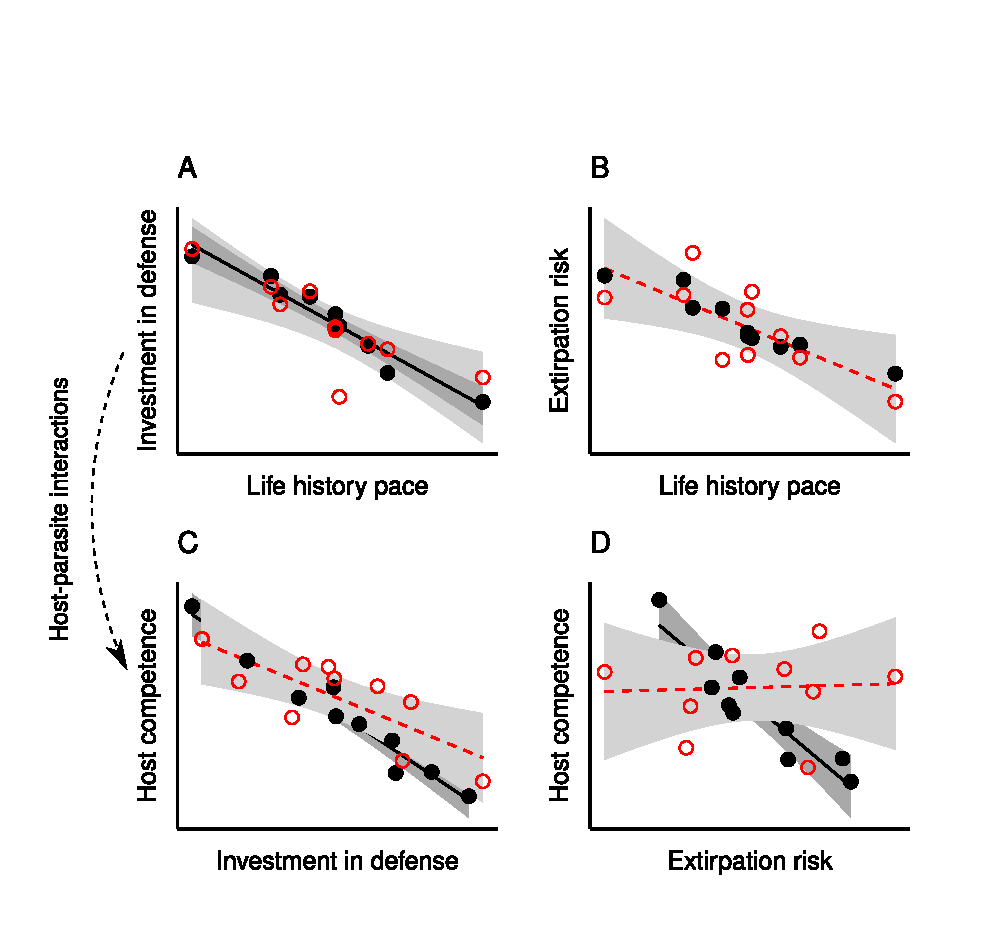
\includegraphics[width=150mm]{figs/ch2/fig1.pdf}
    \end{center}
\label{2-1}
\end{figure}

\begin{figure}
	\caption[Effects of extirpation on disease risk]{
	Split violin plots show the distributions of the effects of extirpations on community R0 across 1000 iterations with deterministic extirpations of large-bodied species in white, and stochastic extirpations with risk proportional to ($1 − w_i^{−1}$) in grey. Red represents amplification (higher community $R_0$ in the more diverse community); blue dilution (lower community $R_0$ in the more diverse community). The leftmost distributions correspond to the identity permutation of intraspecific $R_0$ values (perfect negative rank scaling between extirpation risk and body size) and distributions to the right contain progressively more inversions, until perfect positive rank scaling between host competence and body size is achieved in the rightmost distributions. Intermediate distributions represent a gradient between these two extremes. Horizontal black lines indicate median effects, with surrounding bars showing 25 and 75% quantiles. Here, $a = 3$, $c_{ij} = 0.1$, $k = 0.5$, and $\theta = 1.5$.
	}
    \begin{center}
	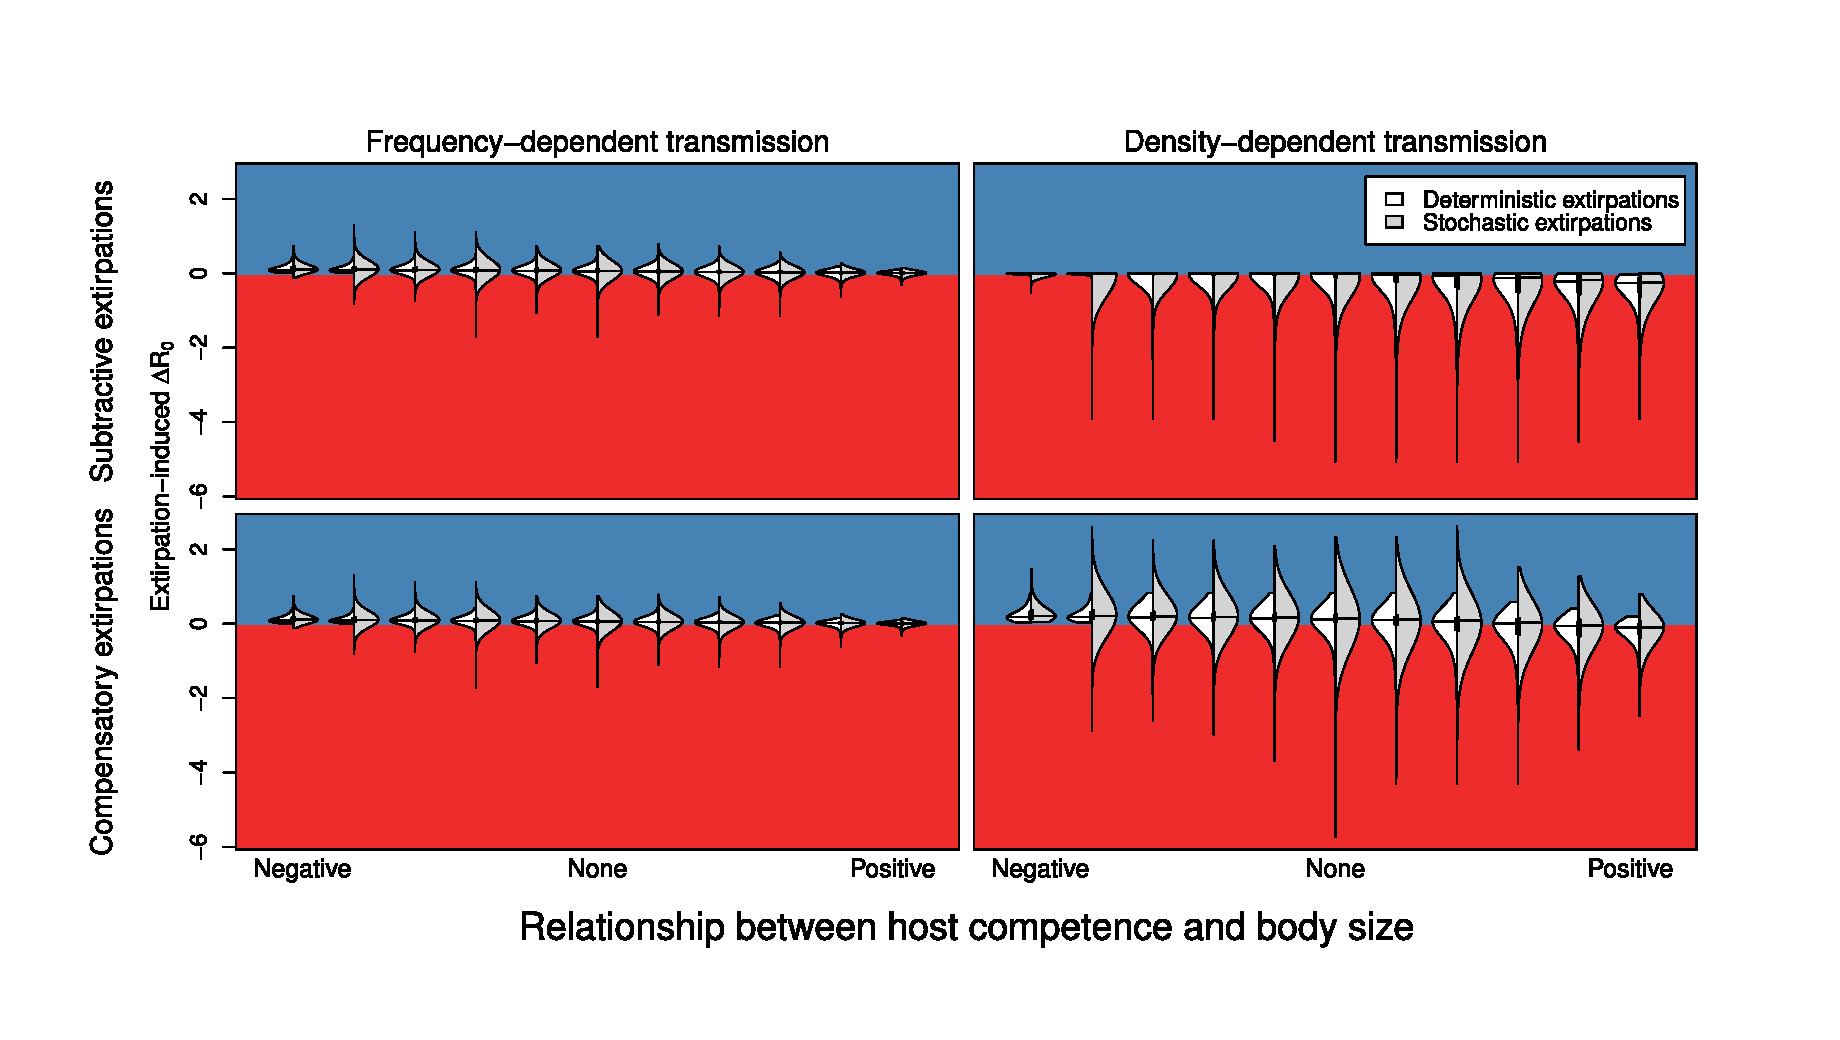
\includegraphics[width=150mm]{figs/ch2/fig2.pdf}
    \end{center}
\label{2-2}
\end{figure}

\begin{figure}
	\caption[Sensitivity to interspecific transmission intensity]{
	Contour plot illustrating variation in the mean effect of species extirpations on community $R_0$ across interspecific transmission strengths and competence-extirpation risk relationships. Larger values of $c_{ij}$ lead to greater interspecific transmission rates (Table \ref{tab2}). Here, large-bodied species are deterministically extirpated, coupling body size with extirpation risk. The x-axis is identical to that of Fig. 2. Numbers along contours denote mean $\Delta R_0$ isoclines, with the zero-isocline marked by a dashed line. Red represents amplification; blue dilution. Here, $a = 3$, $k = 0.5$, $\theta = 1.5$, and $c_{ij}$ was varied from 0.01 to 0.99.
	}
    \begin{center}
	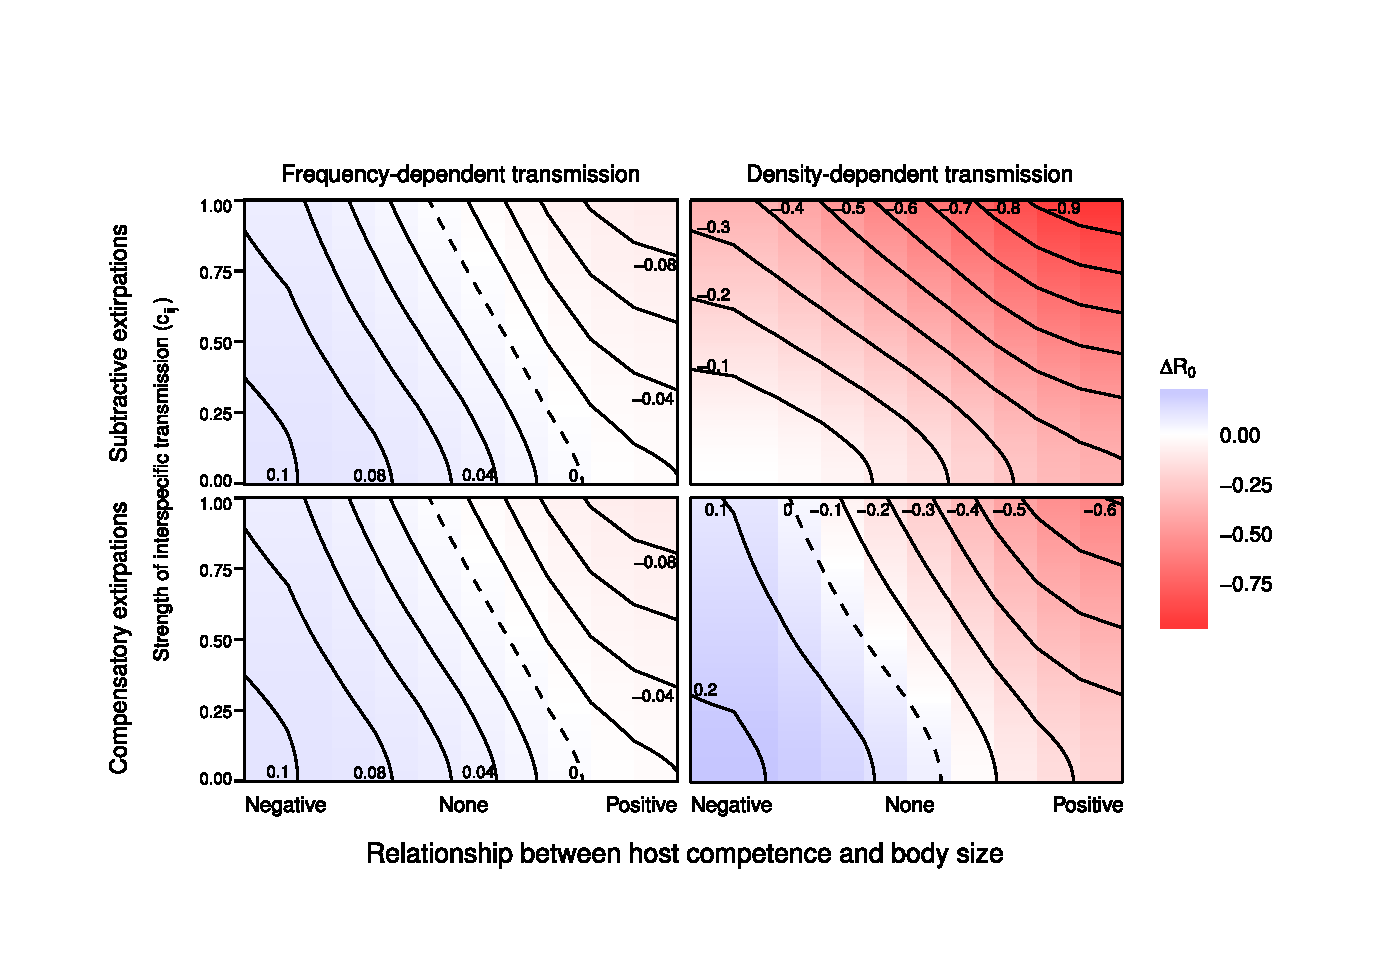
\includegraphics[width=150mm]{figs/ch2/fig3.pdf}
    \end{center}
\label{2-3}
\end{figure}

\begin{figure}
	\caption[Strict allometric scaling between individual weight and intraspecific transmission rate]{
	Line graph depicting relationships between transmission and weight across iterations employing strict scaling (smaller bodied organisms always transmit at a higher rate).
	}
    \begin{center}
	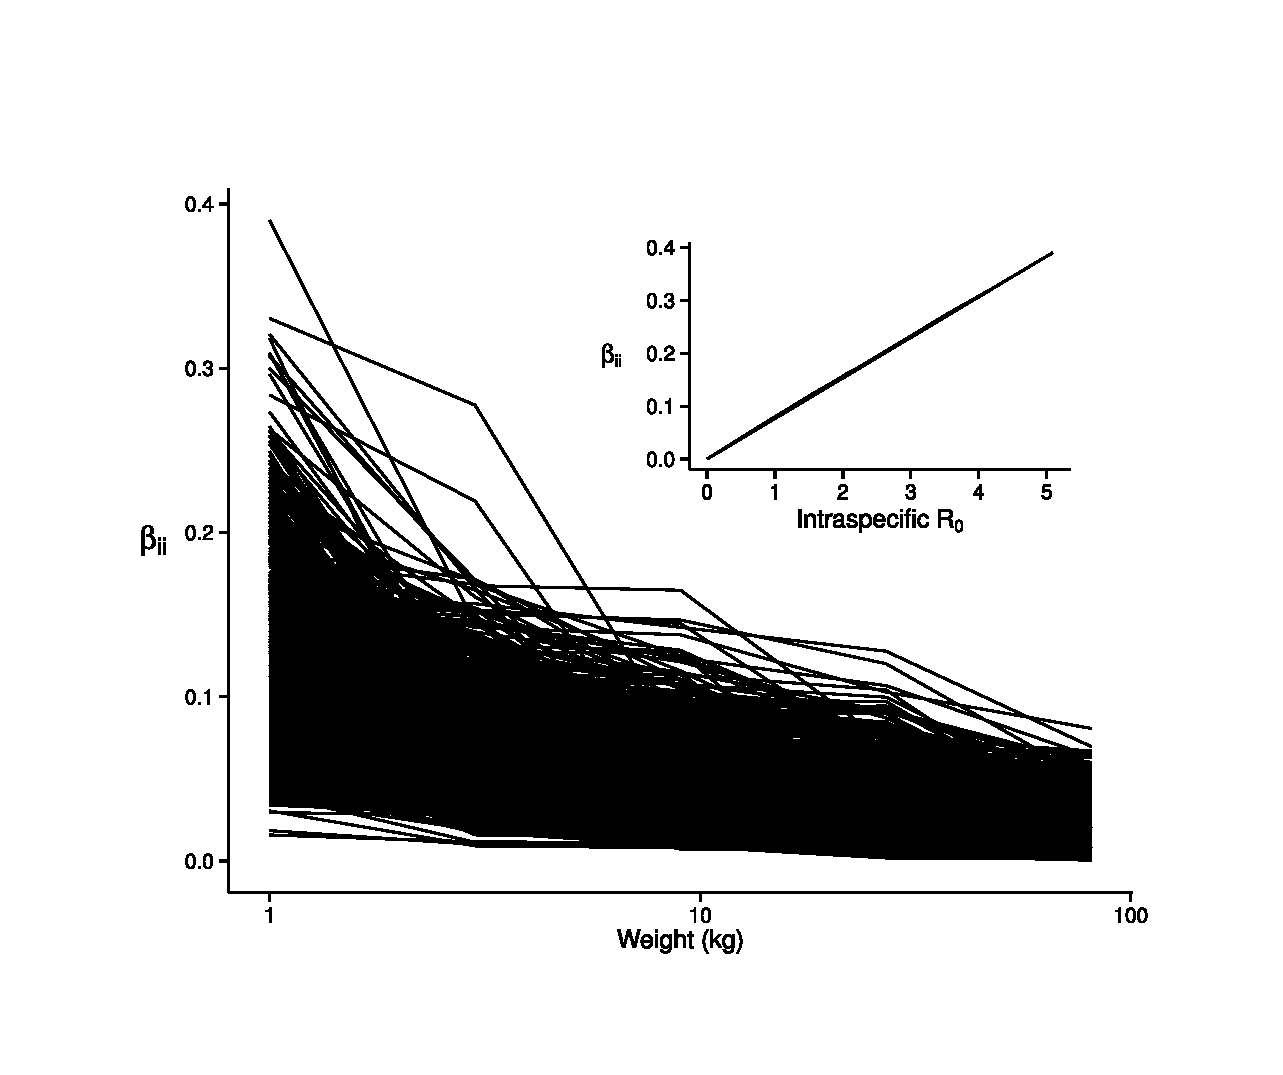
\includegraphics[width=150mm]{figs/ch2/figS1.pdf}
    \end{center}
\label{2-s1}
\end{figure}

\begin{figure}
	\caption[Relaxed allometric scaling between individual weight and intraspecific transmission rate]{
	Scatter plots with overlaid linear regression lines depicting the range of relationships between transmission and weight across iterations as a function of the number of inversions in transmission-weight tuples.
	}
    \begin{center}
	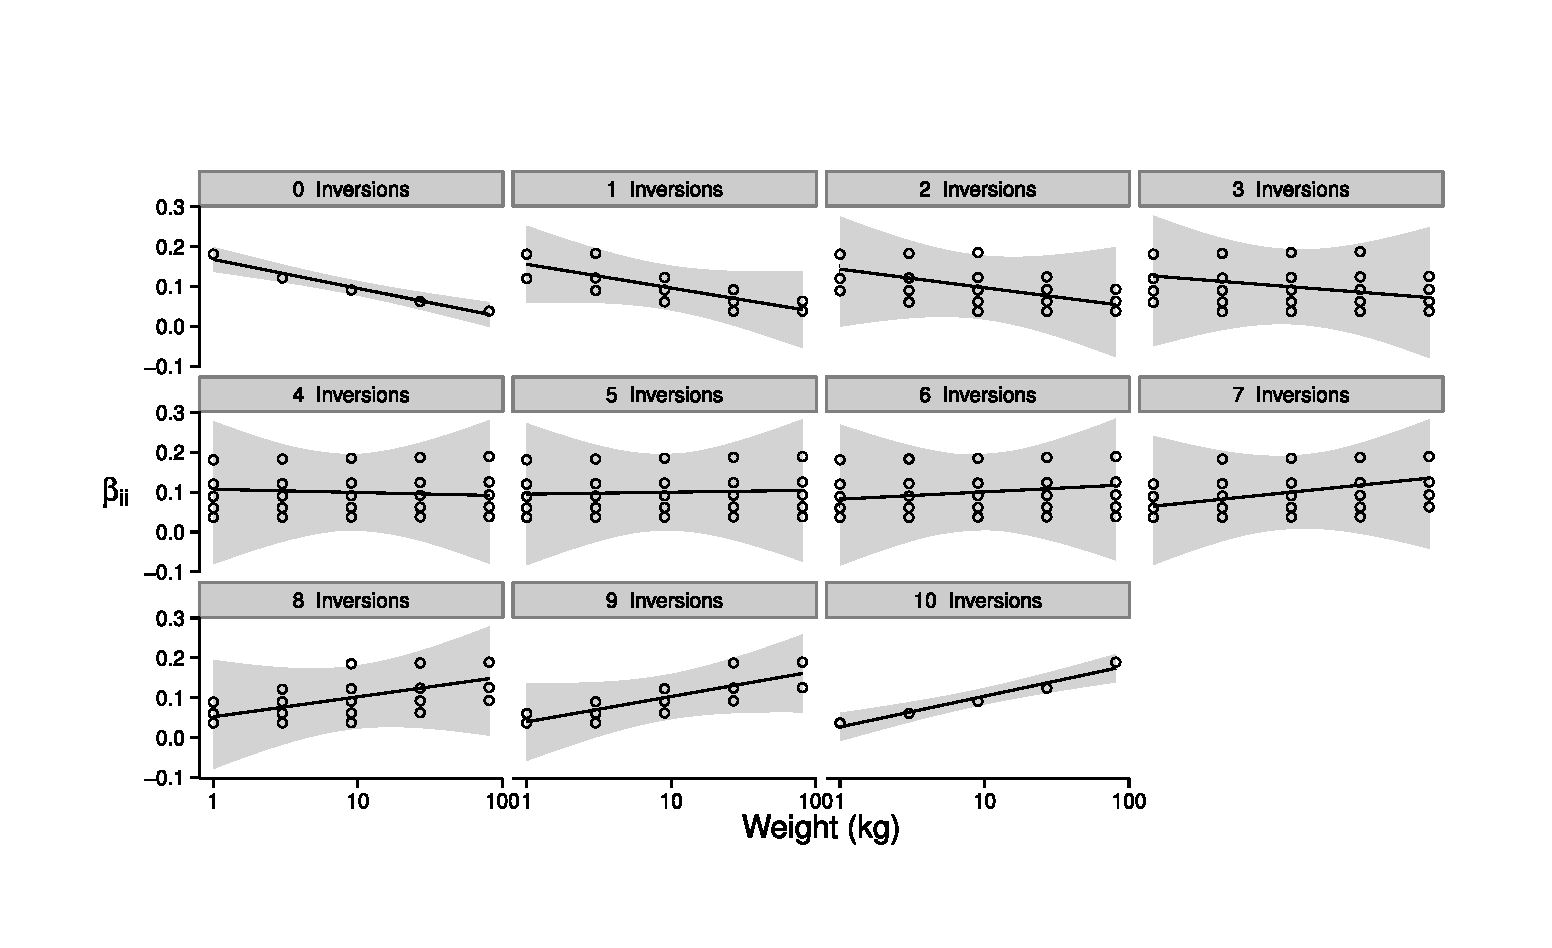
\includegraphics[width=150mm]{figs/ch2/figS2.pdf}
    \end{center}
\label{2-s2}
\end{figure}

\begin{figure}
	\caption[Effects of extirpation on disease risk with random extictions]{
	Split violin plots show the distributions of the effects of extirpations on community R0 across 1000 iterations with deterministic extirpations of large-bodied species in white, and totally random extirpations in grey. Red represents amplification (higher community $R_0$ in the more diverse community); blue dilution (lower community $R_0$ in the more diverse community). The leftmost distributions correspond to the identity permutation of intraspecific $R_0$ values (perfect negative rank scaling between extirpation risk and body size) and distributions to the right contain progressively more inversions, until perfect positive rank scaling between host competence and body size is achieved in the rightmost distributions. Intermediate distributions represent a gradient between these two extremes. Horizontal black lines indicate median effects, with surrounding bars showing 25 and 75% quantiles. Here, $a = 3$, $c_{ij} = 0.1$, $k = 0.5$, and $\theta = 1.5$.
	}
    \begin{center}
	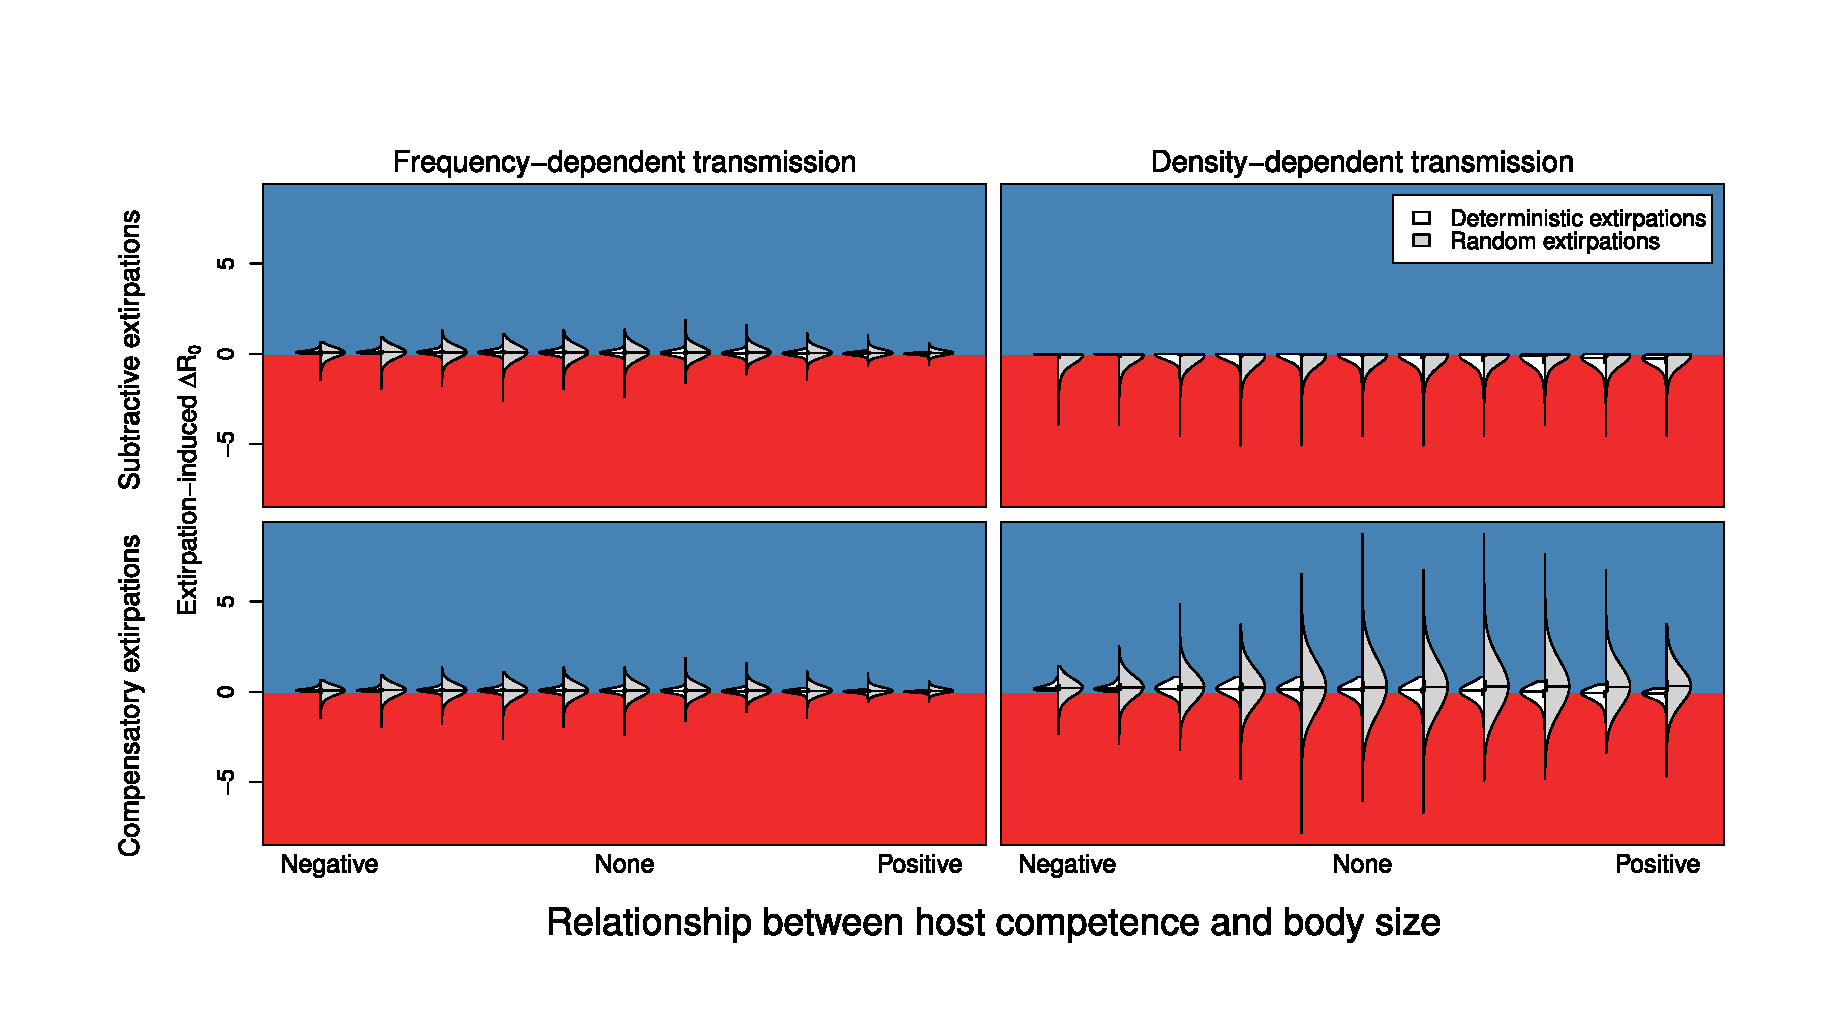
\includegraphics[width=150mm]{figs/ch2/figS3.pdf}
    \end{center}
\label{2-s3}
\end{figure}

\begin{figure}
	\caption[Effect of body size scaling on disease outcomes]{
	Contour plot showing the sensitivity of model predictions to the body size scaling parameter. Solid lines represent $\Delta R_0$ isoclines as in \ref{2-3}.
	}
    \begin{center}
	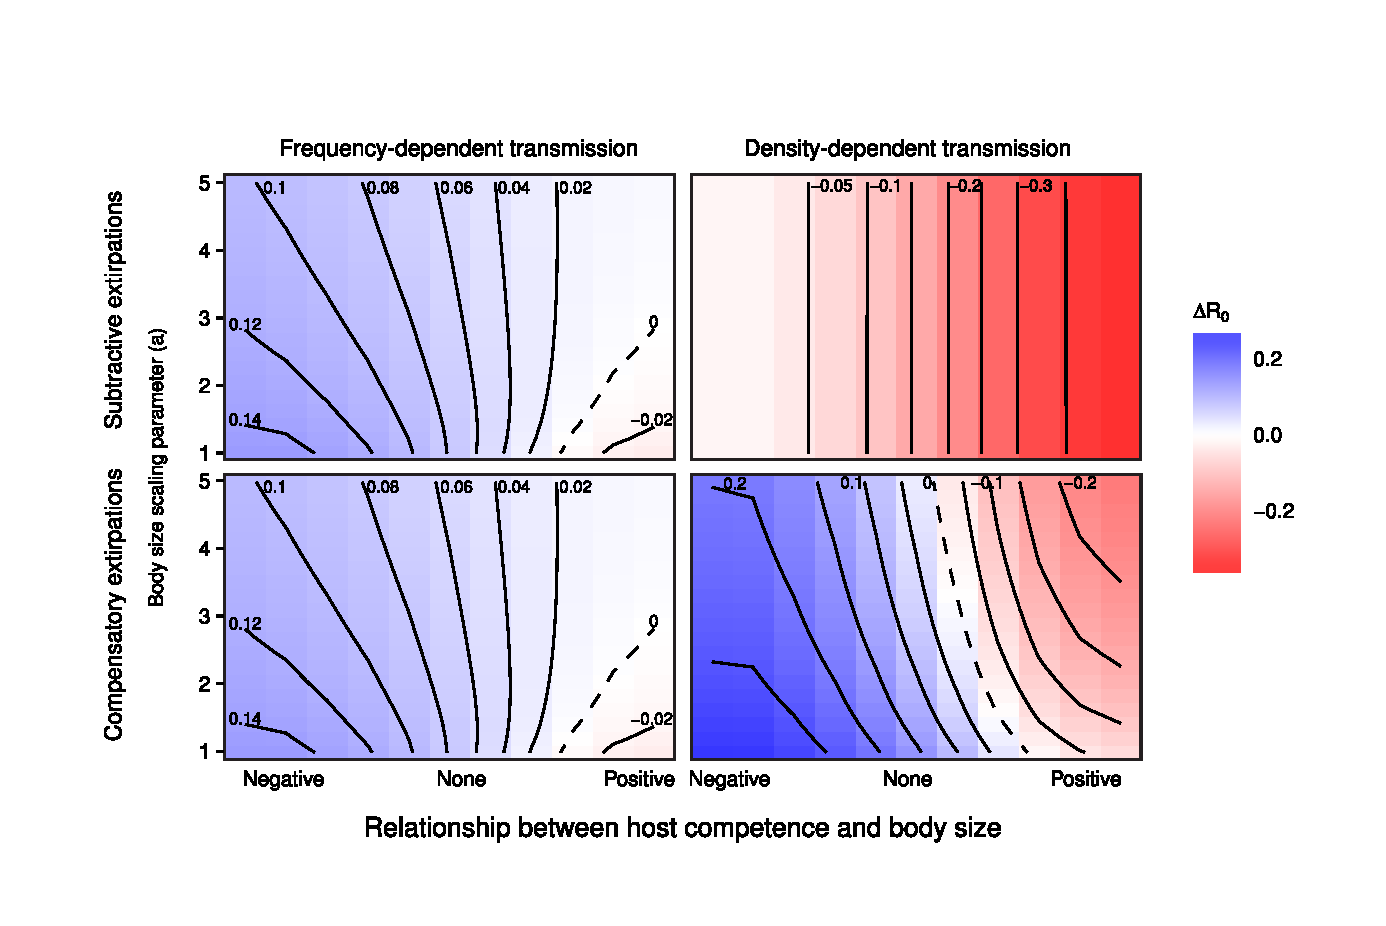
\includegraphics[width=150mm]{figs/ch2/figS4.pdf}
    \end{center}
\label{2-s4}
\end{figure}

\begin{figure}
	\caption[Sensitivity to $R_0$ generative distributions]{
	Model sensitivity to the distribution of $R_0$ values among species. We chose from among three different truncated gamma distributions with varying means and variance.
	}
    \begin{center}
	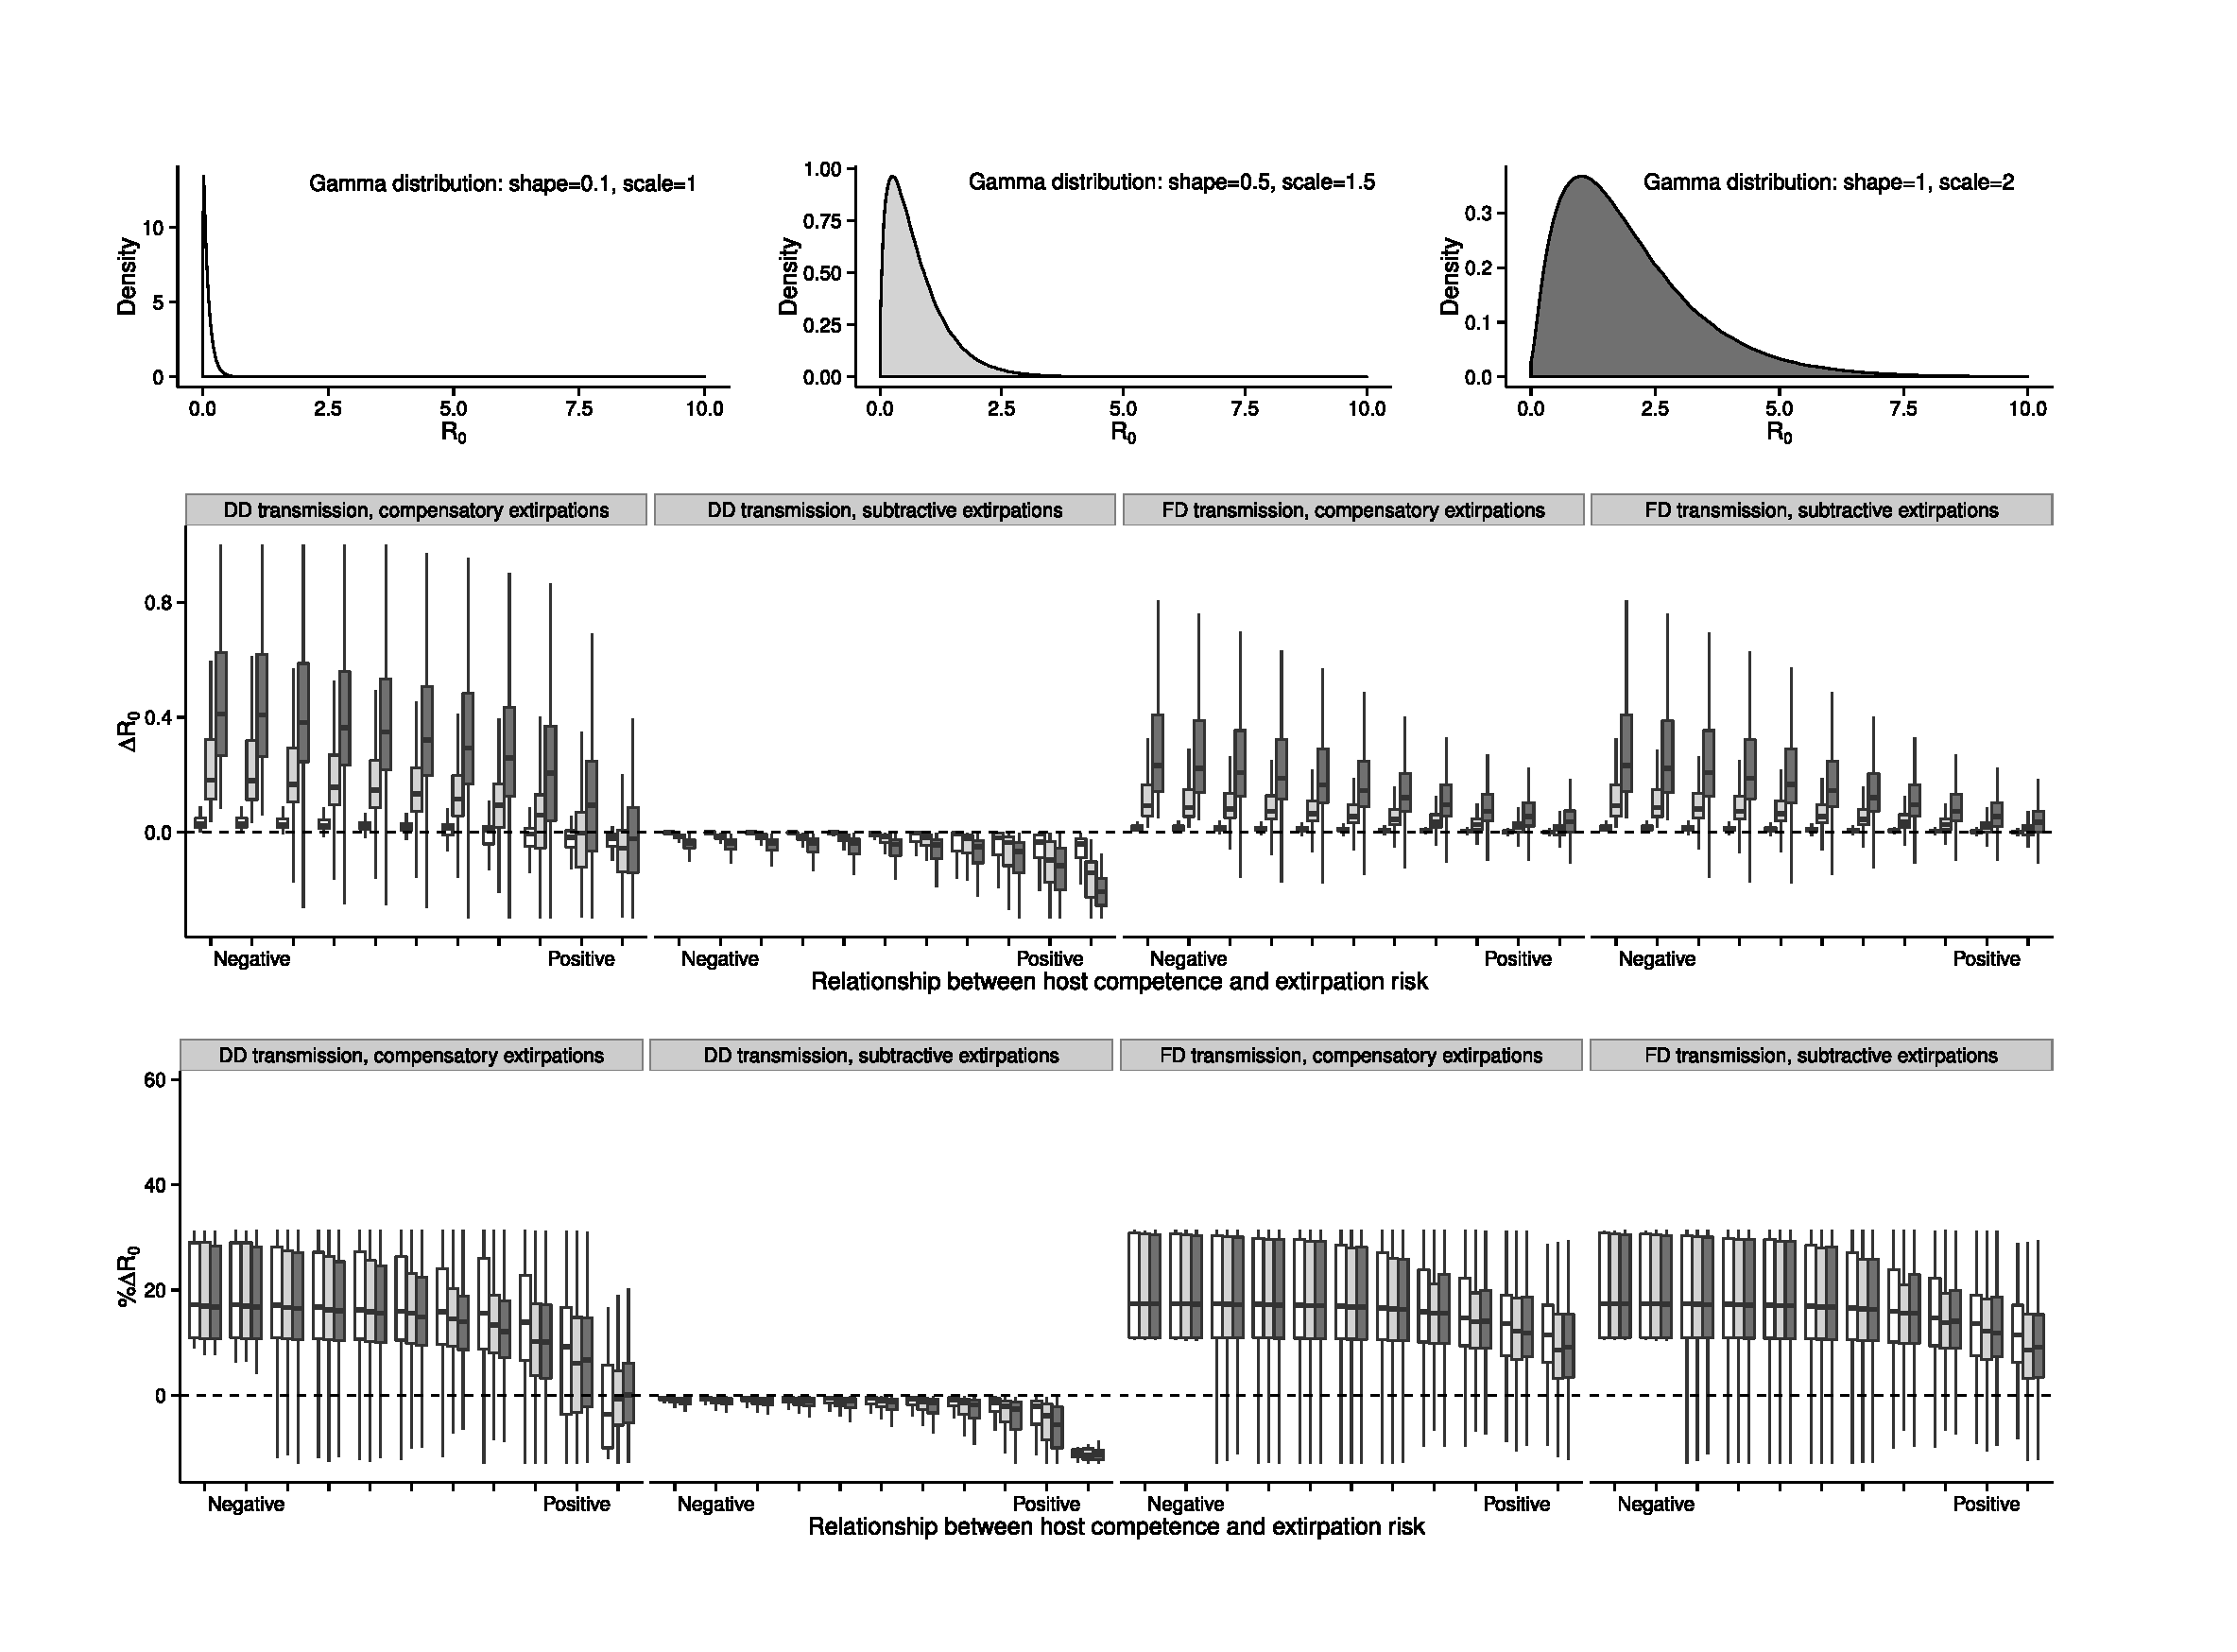
\includegraphics[width=150mm]{figs/ch2/figS5.pdf}
    \end{center}
\label{2-s5}
\end{figure}

\begin{table}
		\centering
		\small
    \caption{
Parameter definitions
	}
    \begin{tabular}{{|p{2cm}|p{8cm}|p{4cm}|}} \hline
	Parameter & Definition & Value \\  \hline \hline
	$w_i$ & Body mass of species $i$ (kg) & $a w_{min}^{i-1}$ \\ \hline
	$w_{min}$ & Minimum species body mass & 1 kg \\ \hline
	$a$ & Weight scaling parameter & varied from 1 to 5 \\ \hline
	$b_i$ & Per capita birth rate & $0.6 w_i^{-0.27} + 0.4 w_i^{-0.26}$ \\ \hline
	$d_i$	& Per capita death rate & $0.4 w_i^{-0.26}$ \\ \hline
	$K_i$ & Carrying capacity	& $(b_i - d_i) / \delta$ \\ \hline
	$\delta$ & Density dependence intensity parameter &	0.01 \\ \hline
	$v_i$ & Infection-induced mortality rate & $(m-1)d_i$ \\ \hline
	$m$	& Virulence term & 1.5 \\ \hline
	$\sigma_i$	& Recovery rate	& $rd_i$ \\ \hline
	$R_{0i}$ & Intraspecific pathogen reproductive ratio	& $\text{Gamma}(k, \theta) \in (0, 10)$ \\ \hline
	$k$	& Gamma shape parameter & varied from 0.1 to 1 \\ \hline
	$\theta$	& Gamma scale parameter & varied from 1 to 2 \\ \hline
	$\beta_{ii}$ & Intraspecific transmission rate & $K_i^{-1} R_{0i} (d_i + v_i + \sigma_i)$\\ \hline
	$\beta_{ij}$ & Interspecific transmission rate & $c_{ij} \dfrac{\beta_{ii} \beta_{ij}}{2}$\\ \hline
	$c_{ij}$ & Interspecific transmission scaling parameter & varied from 0.01 to 0.99 \\ \hline
	\end{tabular}
\label{tab2}
\end{table}
